\chapter{Measuring and control devices}
\begin{overview}
The different issues surrounding the measurement and implementation of an analog control system is discussed. This includes the filtering of noise, the analysis of instrument error and a generic procedure for the calibration of the instrument. 

A theoretical discussion on cold junction compensation  for thermocouple measurement is also given.  
\end{overview}

\section{Noise and filtering}
\eindex{Noise} is characterised by high frequency disturbances with a zero net effect on the measurement and arises from a number of sources such as \citep[538]{Seborg89}:
\begin{enumerate}
	\item the measuring device,
	\item electrical equipment such as a.c. power circuits, generators and turbines, 
	\item that inherently part of the process (i.e. boiling liquid level measurement).
\end{enumerate}
The \emph{noise} generated by these sources degrades the signal condition that is used for the control of the process. This will cause a decrease in controller performance, especially for controllers that use an approximation of the derivative error. The \emph{noise} can however be removed from the incoming signal as it contains no valuable information \citep[389]{Marlin00} for control. Noise is mainly reduced by using proper shielding and grounding or \emph{filtering}. 

Two types of filters can be identified \citep[539]{Richardson94} and are \eindex{analog filters} or \eindex{digital filters}. The \emph{analog filters} are implemented as electrical networks and is used to \eindex{condition} (i.e. to remove or minimize the noise) continuous signals. \emph{Digital filters} are implemented as software on the computer and \emph{condition} sampled data signals \citep[539]{Richardson94}. The theory on which both filters are based, are the same although the implementation may differ.

The filter calculation usually employed in the chemical processing industry is a first order lag or \eindex{low pass filter} \citep[390]{Marlin00}. Its operation can be described by an differential equation of the form:
\(\tau_f\frac{dy(t)}{dt} + y(t) = x(t) \)
with $x(t)$ the data to be filtered, $y(t)$ the raw measurement and $\tau_f$ the filter time constant. The equivalent transfer function description is:
\begin{align}
	x(s) &=  \tau_f y(s)s + y(s)  \nonumber \\
	\therefore \quad y(s) &= \frac{1}{\tau_f s + 1}x(s)
\end{align}
The gain of the filter is one as the filter must not influence the measurement other than reducing the high frequency noise. 
	
The discrete implementation of the filter can be derived and is known as an \eindex{exponential filter} \citep[539]{Seborg89}:
\begin{align}
	x_n &= \tau_f \frac{y_n - y_{n-1}}{\Delta t} + y_n  \nonumber \\
	\therefore \quad y_n &= \frac{\Delta t}{\tau_f + \Delta t}x_n + \frac{\tau_f}{\tau_f + \Delta t}y_{n-1}
\end{align}
The general exponential filter can be written by defining:
\(1 - \alpha \stackrel{\Delta}{=} \frac{\tau_f}{\tau_f + \Delta t} \)
to give,
\(y_n = \alpha x_n + (1 - \alpha)y_{n-1} \)

A frequency plot (Bode plot) of the \emph{low pass filter} shows (figure~\ref{fig:digi:digifilter}) how the fact that the magnitude drops rapidly can be used to reduce the effects of noise by ensuring that the filter gain is small at the frequencies where noise is encountered. 

The filter time constant is used to determine the magnitude at the specified frequency. The filter time constant can, for example, be increased to filter lower frequency noise.
	\begin{figure}[htbp]
		\centering
		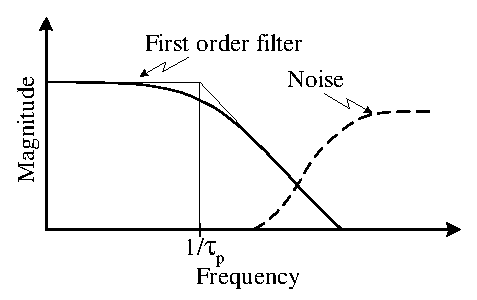
\includegraphics[width = 0.6\textwidth]{digifilter}
		\caption{Low pass filter}
		\label{fig:digi:digifilter}
	\end{figure} 
	
\begin{example}
	A sinusoidal noise measurement with a frequency of 10 rad/s and amplitude of 0.1 is shown in figure 						\ref{fig:digi:boderaw}. A low pass filter can therefore be designed to reduce this noise.
	\begin{figure}[htbp]
		\centering
		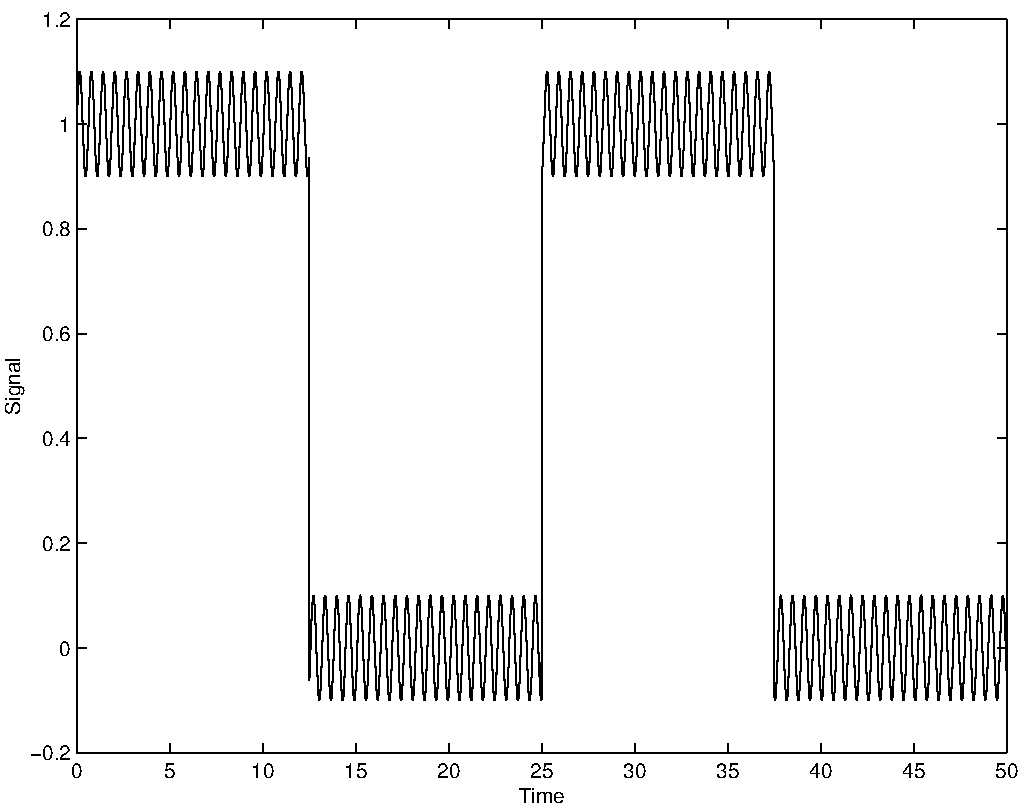
\includegraphics[width = 0.6\textwidth]{digiboderaw}
		\caption{Raw measurement data}
		\label{fig:digi:boderaw}
	\end{figure}
	
	A filter that will reduce the noise by 80\% is developed by firstly specifying the filter gain ($G_f$): 
	\[ \frac{x(s) - y(s)}{x(s)} = 0.8 \]
	\[\therefore \quad G_f = \frac{y(s)}{x(s)} = 0.2\]
	and secondly determine the filter time constant ($\tau_f$), using the magnitude frequency response of the filter transfer function:
	\[G_f = \frac{1}{\sqrt{1 + \omega^2 \tau^2}}\]
	\[\therefore \quad \tau_f = \frac{\sqrt{(\frac{1}{G_f})^2 - 1}}{\omega} = \frac{\sqrt{(\frac{1}{0.2})^2 - 				1}}{10} = 0.5 \]
	to give the low pass filter:
		\[G_{f} = \frac{1}{0.5s + 1} \]
	
	The filter can accordingly be placed in series with the measured data to condition the signal and the 					resultant output signal can be seen in figure~\ref{fig:digi:bodefilter}. 
	\begin{figure}[htbp]
		\centering
		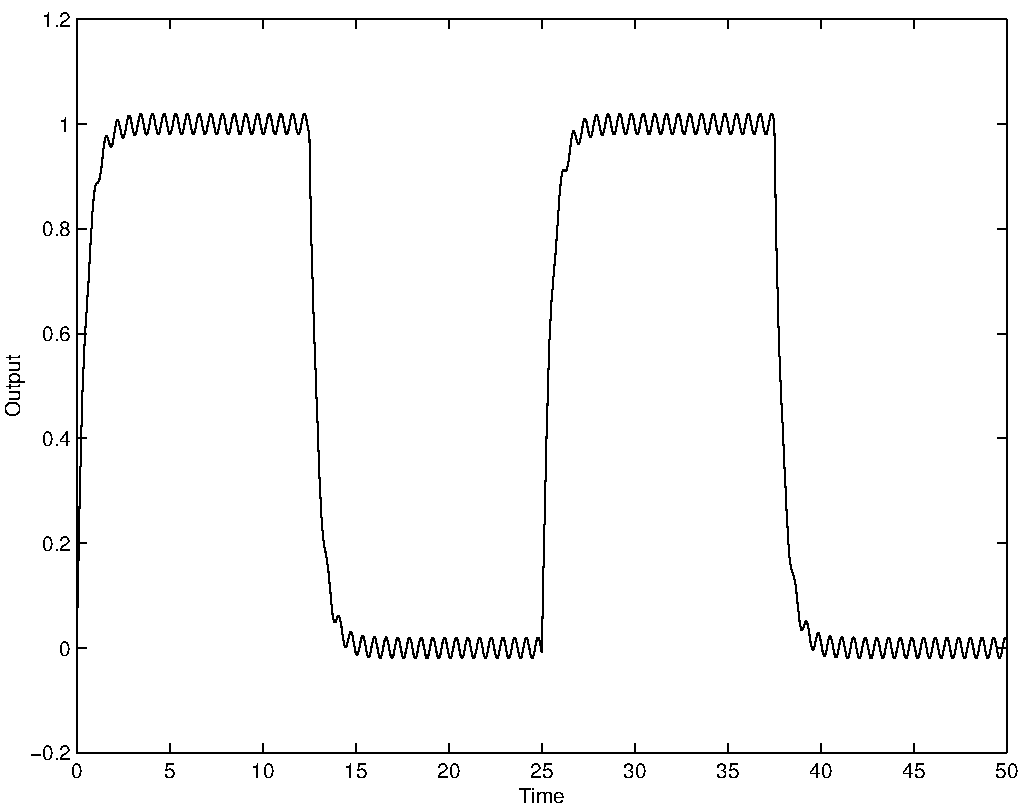
\includegraphics[width = 0.6\textwidth]{digibodefilter}
		\caption{Filtered data}
		\label{fig:digi:bodefilter}
	\end{figure}
	It can be noted that the filter will, however, slow the response of the signal measurement and is slowed more 	as the signal is filtered more. The degradation of the measured signal due to noise and that due to the 				implementation 	of the filter must therefore be optimised. 
	
	Signals used for compressor surge control will, for example, not be filtered as rapid large changes can occur 	that needs immediate action, while level measurement of a storage tank can be filtered more as the process 			dynamics are slow.
\end{example}   

\section{Sensor and actuator calibration}
A sensor or actuator is usually calibrated by adjusting the low range output value or \eindex{zero} as well as the \eindex{span} of the measurement or control. A generic procedure for the calibration of a measuring or control device is given, but it should be noted that the different manuals for the instrumentation should be consulted for more specific details.
\begin{description}
	\item [Step 1:]Set the measured property or the actuator to its minimum input. A tank can, for example, be emptied if a level measurement device is calibrated or a thermocouple can be placed in ice it the temperature measurement is calibrated. The minimum signal output (i.e. 4 mA or 1 VDC) is set by adjusting the ZERO setting of the instrument.
	\item [Step 2:]Set the measured property or the actuator to its maximum input (i.e. fully fill the tank for level measurement calibration) and adjust the RANGE setting to obtain the correct maximum output (i.e. 20 mA or 5 VDC).
	\item [Step 3:]Set the measured property or the actuator to half of its maximum input and check the output to see if the output is linear or non--linear.
	\item [Step 4:]Obtain a mathematical correlation for the sensor or actuator output to the measured property should Step 3 show that the measurement or actuator output is non--linear. This is done by setting the measured property or actuator at different values between the maximum and minimum values and tabulating the corresponding output values.
\end{description}

\section{Sensor and actuator characteristics}
A brief description of the more important characteristics of measurement and control instrumentation, follows. The definitions of theses characteristics is of great importance when deciding on the type of instrument to be purchased, or identifying some current control issues for the task at hand. 

\subsection{Range, span and turndown}
	\begin{description}
		\item{Range} is the region over which a quantity may be measured (input range) or transmitted (output 						range) and is defined by stating the lower and upper range values. \index{range}
 		\item [Span] is the magnitude of the range of the instrument (i.e. the difference between the upper and 					lower range values). \index{span}
		\item [Turndown] is the ratio of the upper range value to the lower range value \citep[529]{Richardson94}. 				\index{turn down}
	\end{description}	

\subsection{Sensitivity}
The \eindex{sensitivity} of a  measuring instrument or actuator is the ratio of the change in magnitude of the output signal corresponding to the change in the magnitude of the input; after a steady state has been reached\citep[529]{Richardson94}. 
\begin{example}
	Consider a typical thermocouple for which the voltage output, $E$, is given by the following expression:
    		\[E = \beta_0 + \beta_1 T + \beta_2 T^2 \]
  where T is the temperature and $\beta$ is the temperature coefficient. The sensitivity of the 									thermocouple can therefore by derived, by differentiation, to obtain:
        \[\frac{dE}{dT} = \beta_1 + 2\beta_2 T \]
  and shows that the sensitivity of this instrument is a linear function of temperature.  	
\end{example}
 
\subsection{Resolution}
\eindex{Resolution} is the minimum difference in the values of a quantity that can be discriminated by a device. Care should be taken to specify instrumentation with the correct  for the application at hand, as more sensitive equipment invariably costs more---but effective control cannot be obtained with a measurement that has a too low \emph{resolution}.

\subsection{Repeatability}
\eindex{Repeatability} gives an indication of the closeness of agreement among a number of consecutive measurements for the same value of input conditions, under the same operating conditions and approached from the same direction for the full range of the instrument \citep[530]{Richardson94}. The direction of approach must be specified as the instrument might have \eindex{hysteresis} where there is a difference in the measurement of the device for the same input condition depending on whether the measurement is increasing or decreasing (figure~\ref{fig:digi:hyst}). 				
\begin{figure}[htbp]
	\centering
	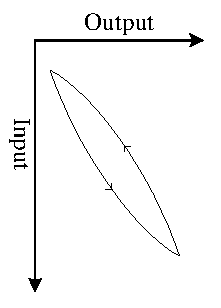
\includegraphics[width = 0.3\textwidth, angle = 90]{digihyst}
	\caption{Hysteresis of a measuring device}
	\label{fig:digi:hyst}
\end{figure}

\subsection{Measurement error}		    
\eindex{Measurement error} of an instrument is the difference between the actual measurement and the true 			value. The measurement error of instrumentation can usually be described with a Gaussian or normal 							distribution that relates the frequency of the error measurement to the measurement error 											(figure~\ref{fig:digi:standard}). 
\begin{figure}[htbp]
	\centering
	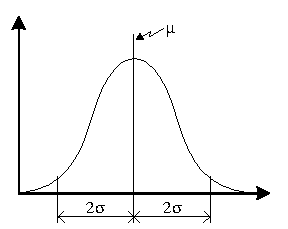
\includegraphics[width = 0.4\textwidth]{digistandard}
	\caption{Standard deviation and confidence intervals of a measuring device}
	\label{fig:digi:standard}
\end{figure}
    		
The \eindex{confidence interval} gives an indication of the maximum deviation expected for a certain 						percentage of measurements. The confidence interval usually used is $\pm$ 2 $\sigma$ from the norm and 					corresponds to 95\% of the measured data readings that is expected to lie within the defined bounds.      
\begin{example}
	The true heights and outputs are tabulated for given a sensor that is used to measure the liquid 								height in a tank. 
	\begin{table}[htbp]
		\centering
  	\caption{Liquid height measurement}
		\begin{tabular}{l c c c c c c c}
			\addlinespace[1em]
			\toprule[1pt]
				Height (cm) & 0 & 5 & 10 & 15 & 20 & 25 & 30 \\
    	\midrule[0.5pt]
    		Output (mA) & 4.1 & 6.3 & 8.9 & 12.5 & 14.5 & 17.1 & 19.8 \\
    	\bottomrule[1pt]
  	\end{tabular}
	\end{table}
The true measurement ($y$) can be calculated if it is assumed that the measured output ($y_m$) of the 					sensor should increase linearly with liquid height ($H$) over a range of 4 to 20 mA.
\begin{align}
	y &=  mH + c \nonumber\\
\therefore \quad y &= 0.53H + 4 \nonumber
\end{align}
The standard deviation ($\sigma$) can then be calculated as a function of the measured ($y_m$) and outputs ($y$), where N is the amount of measured samples \citep[25]{Johnson94}:
\begin{align}
	\sigma^2                  &= \frac{\sum{(y_{m} - y)^2}}{N-1} \nonumber\\
	\therefore \quad \sigma   &= \sqrt{\frac{0.01 + 0.12 + 0.16 + 0.3 + 0.01 + 0.02 + 0.01}{6}} \nonumber\\
	\therefore \quad \sigma   &= 0.33 \nonumber
\end{align}
If it is assumed that the measurement error can be described with a Gaussian distribution, as is the case 			for most measurements, the measurement error can be presented by $y_{m}\pm 2\sigma = y_{m}\pm 0.7 mA$ for 			a 95\% confidence interval. This corresponds to a  3.5\% error margin in the measured output. 
\end{example}

\subsection{Dead band}		
\eindex{Dead band} is the range over which the input to the instrument can be varied without the responding to the output. This a characteristic of control valves that are ``sticking''. A typical response curve for an instrument that has \emph{dead band} can be seen in figure~\ref{fig:digi:dead}.
\begin{figure}[htbp]
	\centering
	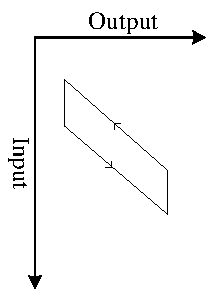
\includegraphics[width = 0.3\textwidth, angle = 90]{digidead}
	\caption{Dead band  response of a measuring device}
	\label{fig:digi:dead}
\end{figure}        

%\section{Measurement descriptions}
%The devices is responsible for the measurement of different properties of the process. This information can be used to infer the control
%actions that must be taken. The measurement usually contains two parts, viz. a \eindex{sensor} and a \eindex{transmitter}
%\citep[200]{Seborg89}. The \emph{sensor} converts the measured property into a useful electrical signal while the \emph{transmitter} will: 
%\begin{itemize}
%	\item convert the signal to a suitable standard (4--20 mA or 1--5 VDC),
%	\item power the sensor (if needed) and,
%	\item filter the incoming signal from the sensor.
%\end{itemize}
%The two parts can be combined in one instrument, which is termed a \eindex{transducer} \citep[437]{Richardson94}, or be two different devices.
%The different types of sensor measurement is discussed further.

\section{Cold junction compensation}
\subsection{Background}
Two materials (X and Y) with different thermo-electric properties will generate a potential difference, termed a \eindex{Seebeck voltage}, if the two junctions of the materials are at different temperatures (figure~\ref{fig:digi:thermo}). This thermo-electric effect can be used to infer temperature by measuring the potential difference ($E_{XY}$). 
\begin{figure}[htbp]
	\centering
	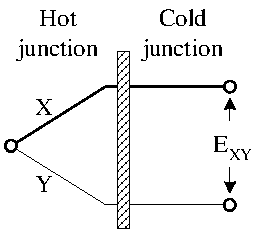
\includegraphics[width = 0.3\textwidth]{digithermo}
	\caption{Thermocouple description}
	\label{fig:digi:thermo}
\end{figure}

Five laws of thermocouple behaviour can be listed \citep[469]{Richardson94}:
\begin{enumerate}
	\item The emf depends only on the temperatures of the junctions and is independent of the temperatures of the 		wires connecting the junctions. The leads that joins the measurement (hot) and the reference (cold) 						junction may experience temperature fluctuations without effecting the reading.
	\item If a third metal Z is inserted between X and Y then, provided that the two new junctions are at the 				same temperature the emf is unchanged. A measuring device such as a voltmeter can be placed in the 							circuit without affecting the emf. 
	\item If a third metal Z is inserted between X and Y then, provided that the new junctions XY and ZY are both 		at the same temperature the emf is the same. The connections can accordingly be soldered or brazed.   
	\item If the emf obtained using the metals X and Y is $E_{XY}$ and that using metal Y and Z is $E_{YZ}$ the 			emf obtained employing X and Z will be (Law of intermediate materials):
				\(E_{XY} = E_{XY} + E_{YZ} \)
	\item If a thermocouple produces a emf $E_{XY}^{T_1 , T_2}$ when its junctions are at $T_1$ and $T_2$ 						respectively and $E_{XY}^{T_2, T_3}$ when its junctions are at $T_2$ and $T_3$ then it will produce and emf 		(Law of intermediate temperatures):
				\(E_{XY}^{T_1 , T_3} = E_{XY}^{T_1 , T_2} + E_{XY}^{T_2 , T_3}\)
		when the junctions are at $T_1$ and $T_3$. This property is used extensively for thermocouple compensation.
\end{enumerate}

\subsubsection{Thermowell}
The thermocouple must be protected against the abrasive materials that is measured. The thermocouple is subsequently placed in a \eindex{thermowell} (figure~\ref{fig:digi:thermowell}) to protect the thermocouple. It should be noted that the thermowell will influence the temperature measurement. 
\begin{figure}[htbp]
	\centering
	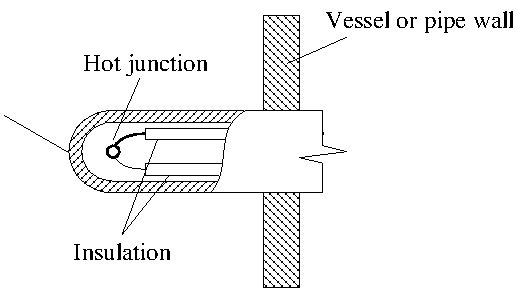
\includegraphics[width = 0.5\textwidth]{digithermowell}
	\caption{Thermocouple placed inside a thermowell}
	\label{fig:digi:thermowell}
\end{figure}

\subsubsection{Thermocouple compensation}
The thermocouple reading (emf) is a function of both the measurement ($T_1$) and reference ($T_2$) temperatures (i.e. emf = $E_{XY}^{T_1 , T_2}$). The a change in $T_2$ will therefore have an effect on the emf and will subsequently cause measurement errors. $E_{XY}^{T_1 , T_2}$ must accordingly be compensated for, by negating the effect of ($T_2$). This is accomplished through the use of the Law of intermediate
temperatures that can be written for the reference temperature:
 	\(E_{XY}^{T_1 , 0} = E_{XY}^{T_1 , T_2} + E_{XY}^{T_2 , 0}\)
where $E_{XY}^{T_2 , 0}$ varies with the reference temperature ($T_2$), that is usually another thermocouple reading (i.e. the measurement and reference temperatures are the same to give an emf = $E_{XY}^{T_2 , 0}$).

The implementation of an automatic reference junction compensator circuit can be seen in figure~\ref{fig:digi:comp}. The compensation can be implemented in the electrical circuit (i.e. reference emf is connected in series with the reading) but is inefficient if a large number of thermocouple is used as each of the readings must be compensated for on the electrical circuit. 
\begin{figure}[htbp]
	\centering
	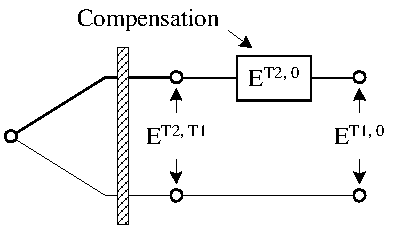
\includegraphics[width = 0.4\textwidth]{digicomp}
	\caption{Thermocouple compensation configuration}
	\label{fig:digi:comp}
\end{figure}
A more efficient configuration for a system that uses a large number of thermocouples is to do the compensation with software (i.e. the measurement emf is added to the reference emf reading).
   
%\subsection{Resistive temperature detector}
%The \eindex{resistive temperature detector} or RTD utilises the fact the resistance of a component changes with a change in temperature and can be expressed by \citep{Richardson94}:
%	\( R_x = R_0 (1 + \beta_1 T + \beta_2 T^2 + \cdots + \beta_N T^N)\)
%where $R_0$ is the resistance a 0 $^\circ{C}$ and $\beta$ are temperature coefficients of resistance.

%\subsubsection{Wheatstone bridge}
%The resistance measurement is transformed to a voltage measurement by utilising a \eindex{Wheatstone bridge}. The simplified bridge configuration can be seen in figure~\ref{fig:digi:bridge}.
%\begin{figure}[htbp]
%	\centering
%	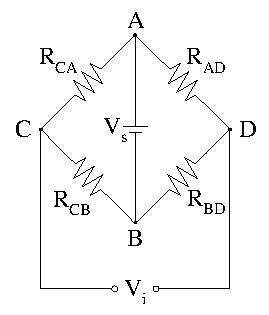
\includegraphics[width = 0.3\textwidth]{digibridge}
%	\caption{General Wheatstone bridge configuration}
%	\label{fig:digi:bridge}
%\end{figure}
%The measured voltage ($V_i$) can be given as a function of the supply voltage ($V_0$) and resistors ($R$):
%\begin{align}
%	V_{AB} &= (R_{CB} + R_{CA})I_{CB}\\
%	\mathrm{but~}\qquad I_{CB} &= \frac{V_{CB}}{R_{CB}}\\
%	\therefore \qquad V_{CB} &= V_{AB}\frac{R_{CB}}{(R_{CA} + R_{CB})}    
%\end{align}
%It can also be shown by the same calculation that:
%	\( V_{BD} = V_{AB}\frac{R_{BD}}{(R_{AD} + R_{BD})}\)
%But $V_i = V_{CB} - V_{AB}$ and $V_{AB} = V_s$
%	\(\therefore \qquad \frac{V_i}{V_s} = \frac{R_{CB}}{(R_{CA} + R_{CB})} - \frac{R_{BD}} {(R_{AD} + R_{BD})} \label{eq:digi:bridge}\) 
%Equation~\ref{eq:digi:bridge} shows that a change in resistances $R_{CA}$ and $R_{CB}$ will have an influence on the measured voltage
%($V_i$). 

%The bridge configuration is said to be balanced when the measured potential difference is zero (i.e. $V_{CB} = V_{AB}$). The different relationships for the resistors used can accordingly be written as:
%\begin{align}
%	\frac{R_{CB}}{(R_{CB} + R_{CA})} &= \frac{R_{BD}}{(R_{BD} + R_{AD})} \\
%	\therefore R_{CB} &=	R_{CA}\frac{R_{BD}}{R_{AD}} 
%\end{align}
%The bridge can therefore be balanced by adjusting $R_{CB}$ is the other resistances are known.
            
%\subsubsection{Three wire implementation}
%Figure~\ref{fig:digi:rtd} shows the typical three lead measuring circuit for measuring the temperature with the RTD. $R_{CA}$ and $R_{AD}$ is known, while $R_{f}$ is a variable resistance resistor that is used to balance (zero) the bridge. 
%\begin{figure}[htbp]
%	\centering
%	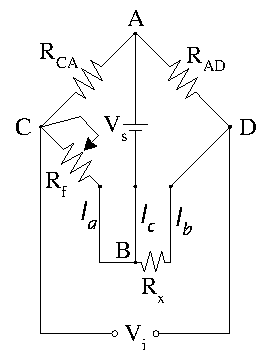
\includegraphics[width = 0.3\textwidth]{digirtd}
%	\caption{Three wire RTD configuration}
%	\label{fig:digi:rtd}
%\end{figure}

%$R_x$ is the variable resistance that changes with temperature. The ambient temperature can influence the measurement. The third wire ($l_a$) is accordingly used for temperature compensation. The circuit balances for a balanced bridge can be written:
%	\(R_{c} + R_{a} + R_{f} + R_{CA} = R_{c} + R_{b} + R_{x} + R_{AD}\)
%but, for a balanced bridge is $V_{CB} = V_{AB}$ or $R_{CA} + R_{f} = R_{AD} + R_{x}$
%	\(\therefore \qquad R_{a} = R_{b}\) 
%Any resistance effects caused by the ambient temperatures will accordingly be negated, if the two wires (a and b) have the same resistance properties ($R_a$ and $R_b$).

%\subsection{pH probe}

%\subsection{Differential pressure probe}

%\subsection{Turbine flow meter}

